% ------------------------------------------------------------------------------
% Preamble
% ------------------------------------------------------------------------------
 
\documentclass[12pt]{article}
 
\usepackage[margin=1in]{geometry} 
\usepackage{amsmath,amsthm,amssymb,enumitem,MnSymbol}
\usepackage{graphicx,filecontents}
\usepackage{hyperref}
 
\newcommand{\N}{\mathbb{N}}
\newcommand{\Z}{\mathbb{Z}}

\renewcommand\qedsymbol{$\blacksquare$}
 
\newenvironment{theorem}[2][Theorem]{\begin{trivlist}
\item[\hskip \labelsep {\bfseries #1}\hskip \labelsep {\bfseries #2.}]}{\end{trivlist}}
\newenvironment{lemma}[2][Lemma]{\begin{trivlist}
\item[\hskip \labelsep {\bfseries #1}\hskip \labelsep {\bfseries #2.}]}{\end{trivlist}}
\newenvironment{exercise}[2][Exercise]{\begin{trivlist}
\item[\hskip \labelsep {\bfseries #1}\hskip \labelsep {\bfseries #2.}]}{\end{trivlist}}
\newenvironment{problem}[2][Problem]{\begin{trivlist}
\item[\hskip \labelsep {\bfseries #1}\hskip \labelsep {\bfseries #2.}]}{\end{trivlist}}
\newenvironment{question}[2][Question]{\begin{trivlist}
\item[\hskip \labelsep {\bfseries #1}\hskip \labelsep {\bfseries #2.}]}{\end{trivlist}}
\newenvironment{corollary}[2][Corollary]{\begin{trivlist}
\item[\hskip \labelsep {\bfseries #1}\hskip \labelsep {\bfseries #2.}]}{\end{trivlist}}

\newlist{pcases}{enumerate}{1}
\setlist[pcases]{
  label=\underline{Case~\arabic*:}\protect\thiscase.~,
  ref=\arabic*,
  align=left,
  labelsep=0pt,
  leftmargin=0pt,
  labelwidth=0pt,
  parsep=0pt
}
\newcommand{\case}[1][]{%
  \if\relax\detokenize{#1}\relax
    \def\thiscase{}%
  \else
    \def\thiscase{~#1}%
  \fi
  \item
}

\begin{filecontents}{biblio.bib}
@article{jacobson,
 author = {Jacobson, V.},
 title = {Congestion Avoidance and Control},
 journal = {SIGCOMM Comput. Commun. Rev.},
 issue_date = {August 1988},
 volume = {18},
 number = {4},
 month = aug,
 year = {1988},
 issn = {0146-4833},
 pages = {314--329},
 numpages = {16},
 url = {http://doi.acm.org/10.1145/52325.52356},
 doi = {10.1145/52325.52356},
 acmid = {52356},
 publisher = {ACM},
 address = {New York, NY, USA},
}
\end{filecontents}

\usepackage[backend=bibtex]{biblatex} %backend tells biblatex what you will be using to process the bibliography file
\bibliography{biblio}
% ------------------------------------------------------------------------------
% Document
% ------------------------------------------------------------------------------
 
\begin{document}
 
\title{CS244, Assignment 2\\TANGRA:\\ Tangra is yet ANother Great Recursive
Acronym}
\author{Hristo Stoyanov\\
stoyanov@stanford.edu\\
\\
Petar Penkov\\
ppenkov@stanford.edu}
 
\maketitle

\section*{Introduction}

Our code is available at \url{https://github.com/renegat96/cs244_lab2}.

\section*{Part A}

The first step of our experiment was to compare the performance of fixed-window
congestion control algorithms while ranging the window size. The values explored
for the congestion window size were the default value of 50 packets and all
powers of 2 from 1 to 64 packets, inclusive. We fixed the timeout to the default
value of 1 second. We found that all values give consistent results with small
noise through multiple runs. Delay and throughput were low for small windows and
big for large windows. Furthermore, the power score improved while increasing
the window size to 16, up to a maximum of 12.21, and it then started to
gradually decline. The results of our experiment are summarized on Figure
\ref{fig:fixed}.

\begin{figure}[h]
 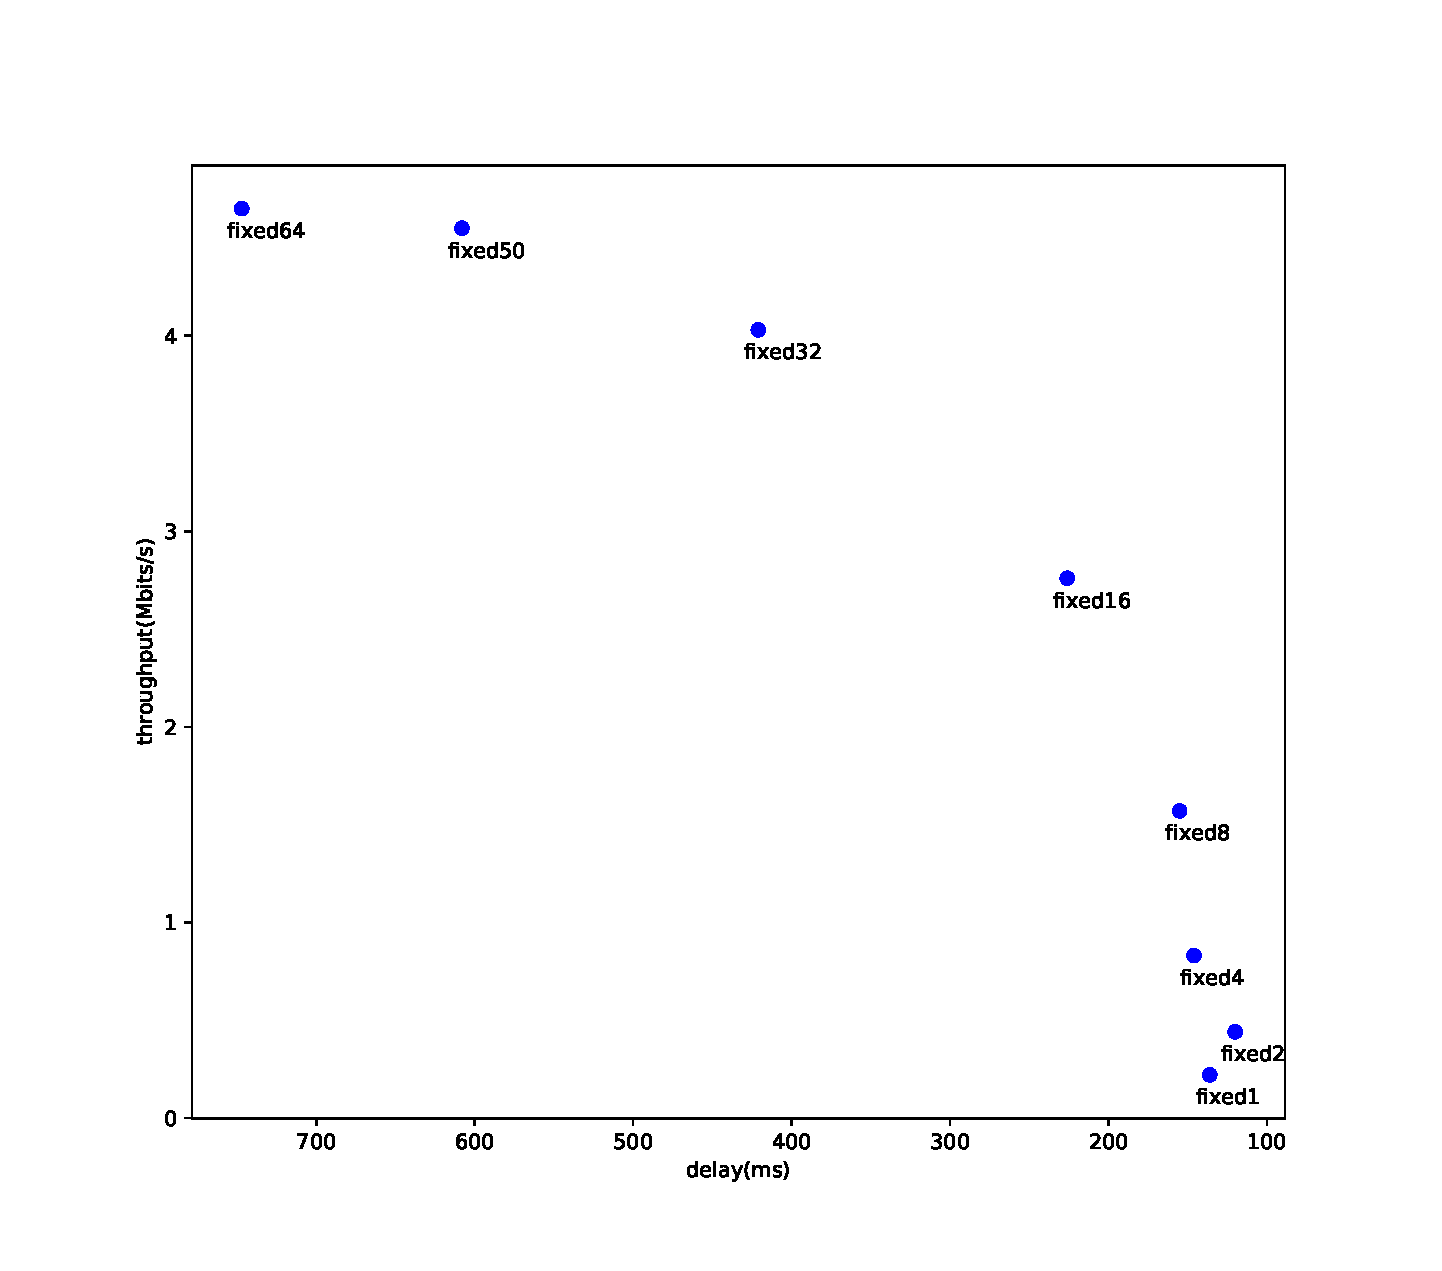
\includegraphics[width=\textwidth,height=\textheight,keepaspectratio]{figure_fixed.eps}
 \caption{A graph of how throughput and delay change as we increase a fixed
 congestion window from 1 to 64 at every power of 2.}
 \label{fig:fixed}
\end{figure}
\section*{Part B}

%REF: V. Jacobson and M. J. Karels, Congestion Avoidance and Control, SIGCOMM 1988.

To capture the variability of link bandwidth, we implemented a simple AIMD
scheme.  Initially we left the timeout fixed to a hardcoded value of 200
milliseconds, but later changed it to be a function of an estimated round-trip
time via a low pass filter, where R is the current estimate and M is the new RTT
measurement on every ACK. \cite{jacobson}

$${RTT} \leftarrow \alpha {RTT} + \left(1 - \alpha\right)M$$

From this estimate of the current RTT we compute the timeout interval to ßR. We
used the suggested parameters $\alpha = 0.9$ and $\beta = 2$. While the
performance of the scheme with a fixed timeout value was consistent [SEE GRAPH
COLOR], there was a significant bufferbloat in the  latter scheme and it was
deemed inadequate.

\section*{Part C}

Our first implementation of a delay-triggered congestion control scheme had two
fixed threshold values. The implementation used a weighted moving average to
estimate the current round-trip-time. If the RTT was below 80ms, the congestion
window is increased, and if the RTT estimate is above 100ms, the window is
decreased.

We experimented with several values of the thresholds, as well as different
values for the increase and decrease of the windows.

\subsection*{Part C1: changing the thresholds}

We attempted to modify the thresholds to different values. Figure 1 shows some
of the results we achieved through picking different values for the low and high
water marks. These include picking 60ms-100ms, 60ms-80ms and 80ms-100ms as
thresholds. This presents a very clear trade-off between delay and throughput.

\subsection*{Part C2: changing the increase/decrease functions}

Further, we tried to change the increase and decrease functions at each crossing
of the thresholds. The best results seemed to be by achieved by using additive
increase and additive decrease. Our increase function was $2/cwnd$. We tried to
use $5/cwnd$ as well, but that did not produce a significant improvement.

\begin{figure}[h]
 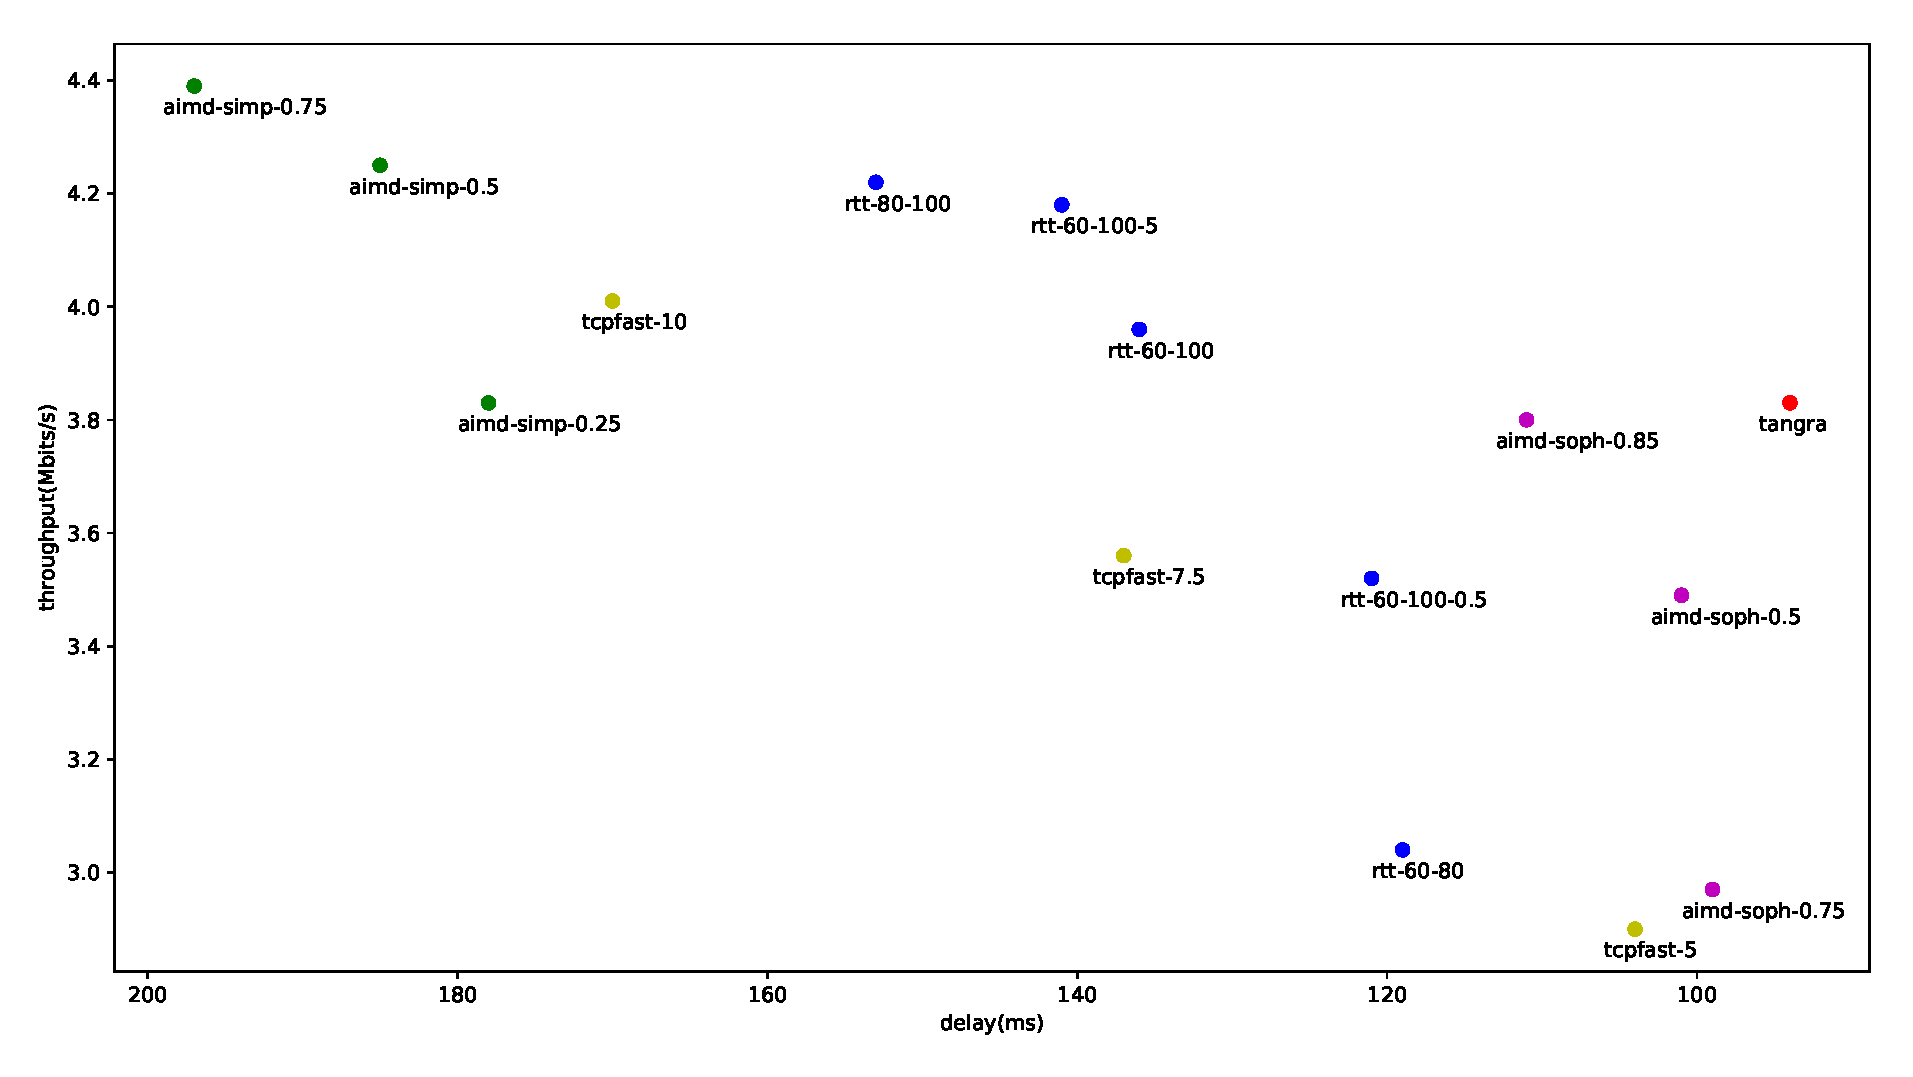
\includegraphics[width=\textwidth,height=\textheight,keepaspectratio]{figure_1.eps}
 \caption{A graph of delay and throughput of different mechanisms.}
 \label{fig:all}
\end{figure}

\section*{Part D}

\subsection*{Part D1: AIMDSoph}

For our use case we found the simple AIMD scheme lacking in two ways. First, the
timeout value of 200ms was hardcoded and would be unreasonable in situations
when just the propagation delay is longer than that. Instead, we set the timeout
to a multiple of the minimum measured round-trip time $RT_{min}$. We found that
a delay of $2*RT_{min}$ works well as it implies queuing delay of one minimum
RTT which is enough to give us feedback while preventing bufferbloat. Second, it
does not account for very small queuing delay. In this case the sender can
probably send more packets. To address this we keep a running estimate of the
RTT via a low pass filter. \cite{jacobson}

$${RTT} \leftarrow \alpha {RTT} + \left(1 - \alpha\right)M$$

Here R denotes the current estimate and M is the measurement on the new ACK. We
use the suggested parameter α = 0.9 to have conservative changes to the current
estimate. For every ACK that maintains the running estimate drops below
$1.5*RT_{min}$, we do another step of additive increase, effectively doubling
the additive increase gain temporarily. Furthermore, to keep the algorithm more
optimistic, we decrease the multiplicative decrease factor from 2 to 1.5 and
double the additive increase gain.

\subsection*{Part D2: TCP Fast}

http://netlab.caltech.edu/publications/FAST-ToN-final-060209-2007.pdf

TCP Fast is a delay-based algorithm that periodically updates the window size
based on the average RTT \cite{jacobson}. <INSERT UPDATE RULE>.

$$cwnd \leftarrow (1 - \gamma)* cwnd + \gamma \left(\frac{cwnd * {RT_{min}}}{RTT} + \alpha \right)$$

The RTT is estimated with the low pass filter function as priorly described, and
the RTTmin is a moving minimum. Additionally, our implementation does not limit
window growth to twice the window size to allow for more aggressive adaptation
to network changes. 

\subsection*{Part D3: TANGRA}

We further developed the idea of RTT-threshold based scheme by incorporating two
more ideas. We first make the assumption that the minimum propagation time does
not change over time. Given this assumption, our algorithm tracks the minimum
RTT and assumes this is the propagation time. Further, we assume that the delay
above the propagation time is proportional to the queueing delay. We write a
control-loop that adjusts the congestion window based on these two assumptions.

The second idea we had was to adjust the congestion window in a way that is
proportional to the difference between the current RTT estimate and a target
RTT. This decision was motivated by the idea that the further away from the
target the current state of the system is, the bigger the correction we need. We
define our target as
$$RTT_{target} \leftarrow t * {RTT}_{min}$$
where $t$ is an adjustable parameter which specifies how big the queuing delay
should be relative to the propagation delay. Our best results are achieved with
$t = 1.4$. In addition, we define $t_{bound}$ and $t_{high}$, as additional
thresholds which will serve to adjust the congestion window. In our default
implementation we used $t_{bound} = 1.6$ and $t_{high} = 1.8$.

This results in 4 levels where the RTT estimate may fall:
\begin{enumerate}
\item $RTT > t_{high} * RTT_{min}$. The current congestion window is
overshooting the target and we need to reduce it drastically.
\item $t_{high}*RTT_{min} >= RTT > t_{bound}*RTT_{min}$. This serves as an
interval where a smaller reduction to the congestion window is applied.
\item $t_{bound} *RTT_{min} >= RTT > t * {RTT_{min}}$. If this condition is
true, the congestion window is not changed.
\item $t * RTT_{min} > RTT$ implies that the current congestion window is too
small, and hence, we increase it.
\end{enumerate}

In order to estimate the $RTT$, we again use a low pass filter, with $\alpha =
0.7$. This may seem too aggressive, but we opted to use that after running
experiments with different values as it provided a trade-off between performance
on the microbenchmark and stability in a network with variance that in RTT over
time. Figure \ref{fig:low-pass-1-4} shows several runs with different low pass
filters.

\begin{figure}[h]
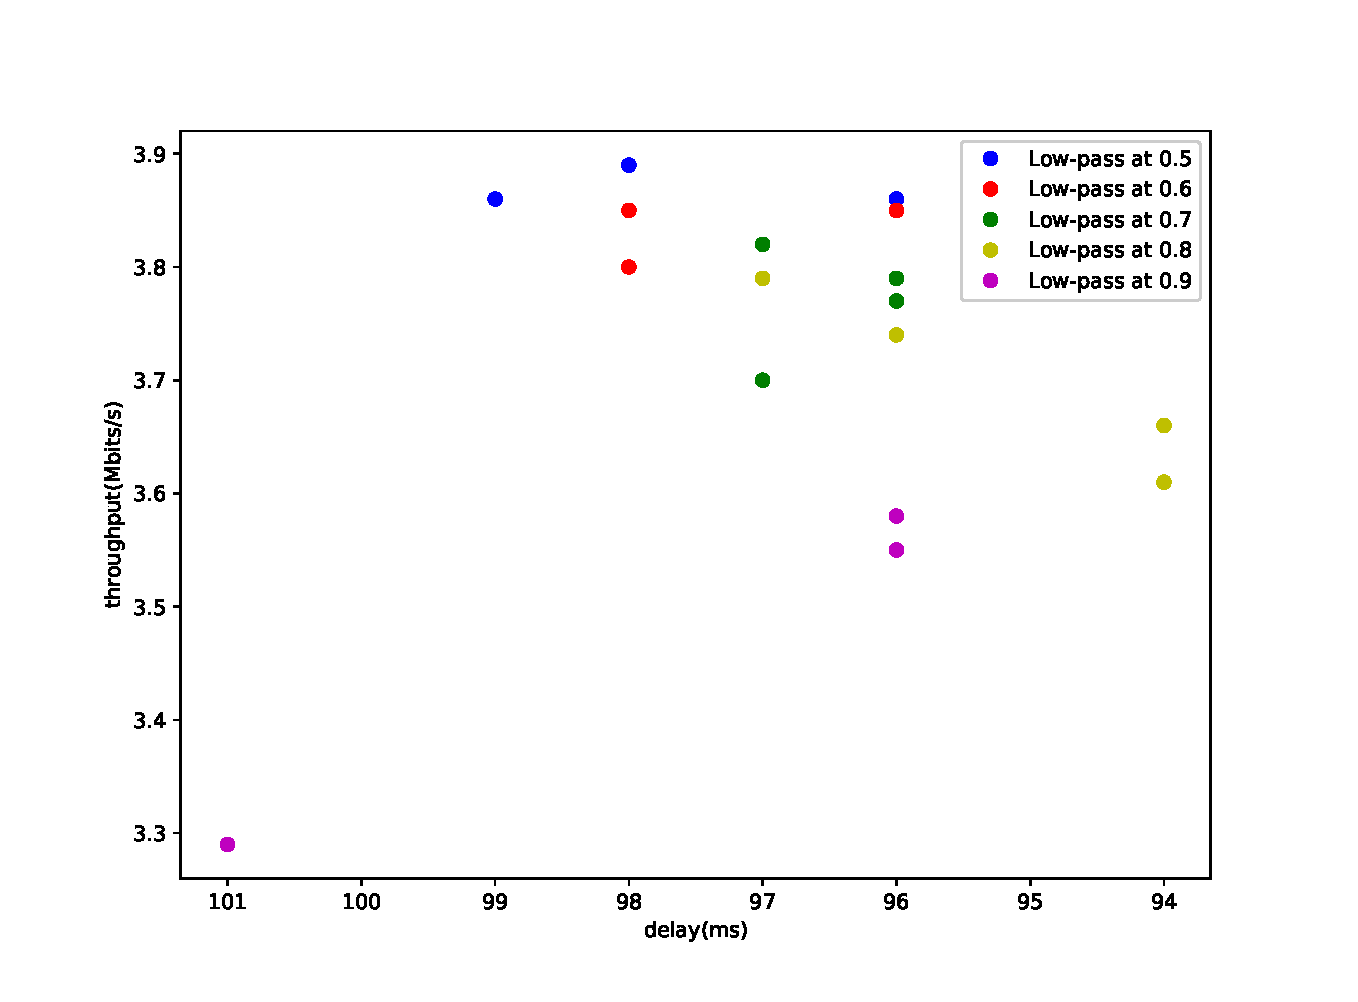
\includegraphics[width=\textwidth,height=\textheight,keepaspectratio]{figure_2.eps}
\caption{Multiple runs of the simulation at $t=1.4$ and different low pass
$\alpha$ parameters.}
\label{fig:low-pass-1-4}
\end{figure}

The best score our implementation achieved was $40.74$ at a throughput of $3.83$
Mbps and 95\textsuperscript{th} percentile signal delay of $94$ ms.

Although our implementation performs very well on this tiny benchmark, this
approach to congestion control has several drawbacks. First, it is very unclear
how several flows will interact with each other. A scenario worth exploring is
where two or more flows share a bottleneck, yet their respective paths are
different and the corresponding proportional queues the flows try to maintain
will be different. This may lead to a much different allocation of the
bottleneck than would otherwise occur with regular TCP.

Another drawback of this approach is the fact that if the $RTT_{target}$ is set
too high relative to the available buffer at the bottleneck link, the algorithm
will likely produce a high loss rate and waste traffic at the links before the
bottleneck by constantly attempting to increase its congestion window.

Future work may be able to address these problems by creating a mechanism to
dynamically adjust the target, while using the same idea of proportionality to
try to hit that target.

\section*{Part E: Naming TANGRA}

Tangra stands for ``Tangra is yet ANother Great Recursive Acronym.'' It also has
a nice ring to it.

\printbibliography

\end{document}
